\documentclass[12pt]{report}
\usepackage[top=3cm, bottom=2.5cm, left=2cm, right=2.5cm]{geometry}
\usepackage{listings}
\usepackage{float}
\usepackage{subfig}
\usepackage{graphicx}
\usepackage{adjustbox}
\usepackage{ptext}
\usepackage[usenames,dvipsnames]{color,xcolor}
\usepackage{xepersian}
\settextfont[Scale=1]{XB Niloofar}
\definecolor{listinggray}{gray}{.98}
\lstset{language=Java,backgroundcolor=\color{listinggray},frameround=fttt,frame=trBL,basicstyle=\ttfamily,keywordstyle=\color{blue}\bfseries,numberstyle=\footnotesize,numbersep=10pt,numbers=left,captionpos=b,breaklines=true,showstringspaces=true}

\title{تمرین سری سوم الگوریتم‌های معاملاتی}
\author{کورش تقی‌پور پاسدار}
\begin{document}
	\maketitle
	\section{توضیح کد نوشته شده}
	در ابتدا مطابق با تصویر زیر، کتابخانه‌ها و داده‌های مربوط به دو رمزارز \lr{Bitcoin} و \lr{Etherium} در دو \lr{interval} یک روزه و پنج روزه در بازه زمانی اول فوریه \lr{2023} تا اول فوریه \lr{2024} لود می‌شوند.
	\begin{figure}[H]
		\centering
		
\includegraphics[scale=0.3]{pic_1}
	\end{figure}
	سپس در کد زیر، نمودار قیمت‌های این دو رمزارز نمایش داده می‌شوند.
	\begin{figure}[H]
		\centering
		
\includegraphics[scale=0.3]{pic_3}
	\end{figure}
	در تصاویر زیر نیز نمودار قیمت‌های رمزارز‌های \lr{BTC} و \lr{ETH} در دو بازه زمانی ۱ روزه و ۵ روزه نمایش داده می‌شود.
	\begin{figure}[H]
		\centering
		\subfloat[
		نمودار قیمت رمزارز \lr{BTC} در بازه‌های زمانی ۱ روزه
		]{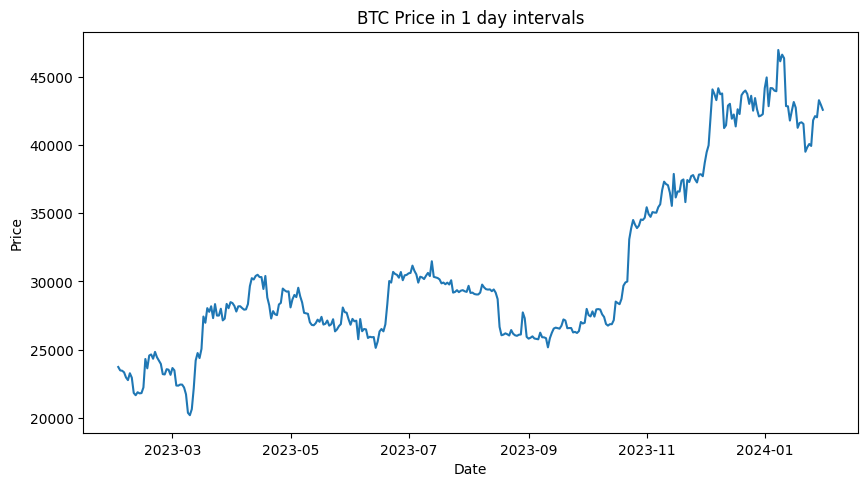
\includegraphics[height=4cm]{pic_2_1}}
		\quad \quad
		\subfloat[
		نمودار قیمت رمزارز \lr{ETH} در بازه‌های زمانی ۱ روزه
		]{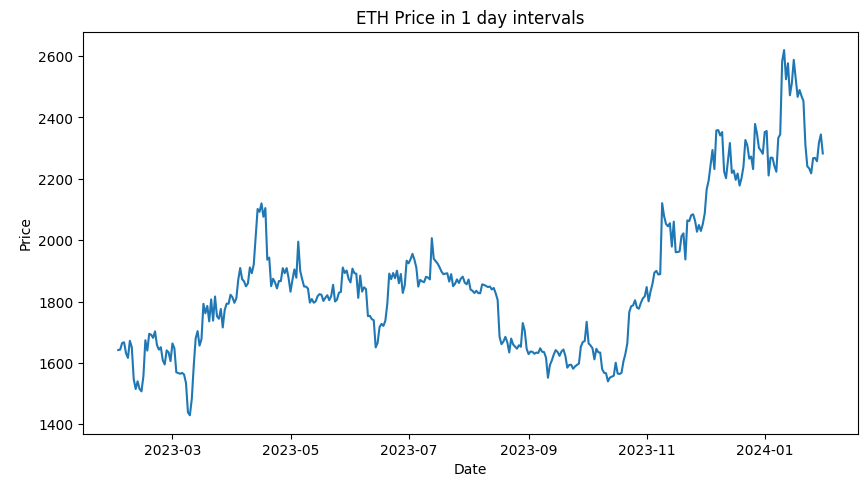
\includegraphics[height=4cm]{pic_2_2}}
		\quad \quad
		\subfloat[
		نمودار قیمت رمزارز \lr{BTC} در بازه‌های زمانی ۵ روزه
		]{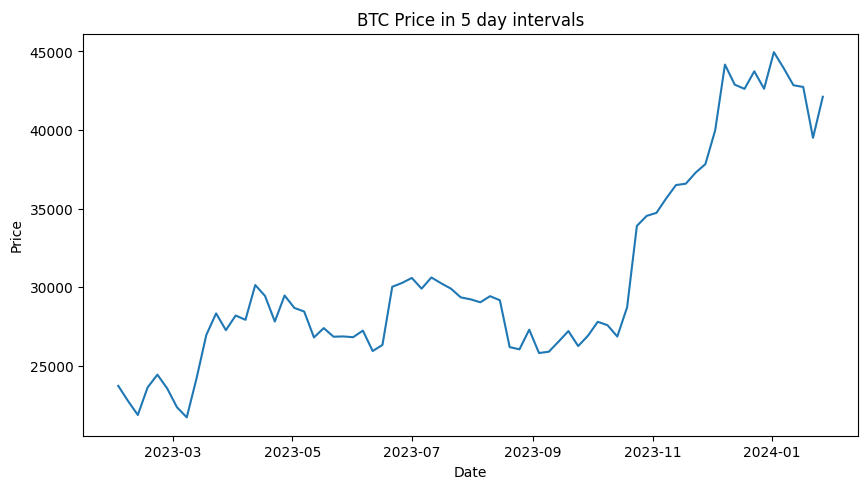
\includegraphics[height=4cm]{pic_2_3}}
		\quad \quad
		\subfloat[
		نمودار قیمت رمزارز \lr{ETH} در بازه‌های زمانی ۵ روزه
		]{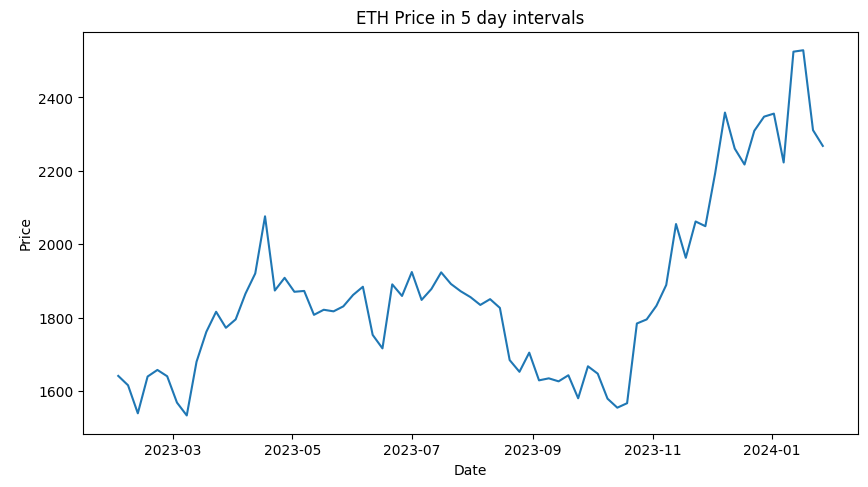
\includegraphics[height=4cm]{pic_2_4}}
	\end{figure}
	در ادامه اندیکاتور \lr{Bollinger Bond} تعریف می‌شود. در این اندیکاتور، ما باند‌های بالایی،‌میانی و پایینی را تعریف و محاسبه می‌کنیم.
	
	باند بالایی از فرمول 
	$$SMA + Std \times Correlation$$
	و باند پایینی از فرمول
	$$SMA - Std \times Correlation$$
	محاسبه می‌شود. همچنین باند میانی با \lr{SMA} برابر است. حال برای محاسبه اندیکاتور \lr{Bollinger Bond}، 
	ما ۴ تابع زیر را تعریف می‌کنیم:
\begin{enumerate}
	\item \textbf{SMA}
	در این تابع، ما \lr{SMA} چند شمع قبلی را حساب می‌کنیم. تعداد این شمع‌ها توسط متغیر \lr{period} تعیین می‌شود.
	\item  \textbf{STD}
	در این تابع، ما انحراف معیار را محاسبه می‌کنیم.
	\item \textbf{UpperBound}
	در این تابع، ما با استفاده از توابع \lr{SMA} و \lr{STD} باند بالایی اندیکاتور را حساب می‌کنیم.
	\item \textbf{LowerBound}
	در این تابع، ما با استفاده از توابع \lr{SMA} و \lr{STD} باند پایینی را حساب می‌کنیم.
\end{enumerate}
در تصویر زیر، پیاده‌سازی اندیکاتور \lr{Bollinger Bond} نشان داده شده است.
\begin{figure}[H]
	\centering
	
\includegraphics[scale=0.5]{pic_4}
	\caption{اندیکاتور \lr{Bollinger Bond}}
\end{figure}
برای نمونه، در تصویر زیر اندیکاتور \lr{Bollinger Bond} برای قیمت \lr{Close} نمودار رمزارز \lr{BTC} در بازه‌های زمانی ۱ روزه نشان داده شده است.
\begin{figure}[H]
	\centering
	
\includegraphics[scale=0.5]{pic_5}
	\caption{اندیکاتور \lr{Bollinger Bond} برای رمزارز \lr{BTC} در بازه‌های زمانی ۱ روزه} 
\end{figure}
حال اندیکاتور \lr{Keltner Channel} تعریف می‌شود. در این اندیکاتور، ما کانال های بالایی و پایینی را بصورت زیر تعریف می‌کنیم.
\begin{eqnarray*}
	Upper Bound &=&SMA + ATR \times Correlation\\
	Lower Bound &=&SMA - ATR \times Correlation
\end{eqnarray*}
همچنین مقدار \lr{ATR} بصورت زیر بدست می‌آید.
\begin{eqnarray*}
	ATR_{init} &=&\frac{\sum^{14}_{i=1} TR_{i}}{14}\\
	ATR_{j+1} &=&\frac{TR_{j} + (n-1)\times ATR_{j}}{n}
\end{eqnarray*}
که در اینجا منظور از \lr{n}، تعداد روزهای دوره است.
حال برای محاسبه باندهای بالایی و پایینی اندیکاتور \lr{Keltner Channel}، ما از توابع زیر استفاده می‌کنیم:
\begin{enumerate}
	\item \textbf{SMA} کارکردی مشابه تابع \lr{SMA} در اندیکاتور \lr{Bollinger Bound} دارد.
	\item \textbf{return\_max} از میان مقادیر $High - Low$، $High - PrevClose$ و $Low - PrevClose$ بیشترین مقدار را انتخاب می‌کند.
	\item \textbf{TR}  به محاسبه مقادیر $High - Low$، $High - PrevClose$ و $Low - PrevClose$ می‌پردازد.
	\item \textbf{ATR} با استفاده از تابع \lr{TR} به محاسبه \lr{ATR} می‌پردازد.
	\item \textbf{UpperBound} با استفاده از مقادیر \lr{sma} و \lr{atr} به محاسبه باند بالایی می‌پردازد.
	\item \textbf{LowerBound} با استفاده از مقادیر \lr{sma} و \lr{atr} به محاسبه باند پایینی می‌پردازد.
\end{enumerate}
حال در تصویر زیر، پیاده‌سازی این اندیکاتور نشان داده شده است.
\begin{figure}[H]
	\centering
	\subfloat[
	قسمت اول تابع اندیکاتور \lr{Keltner Channel}
	]{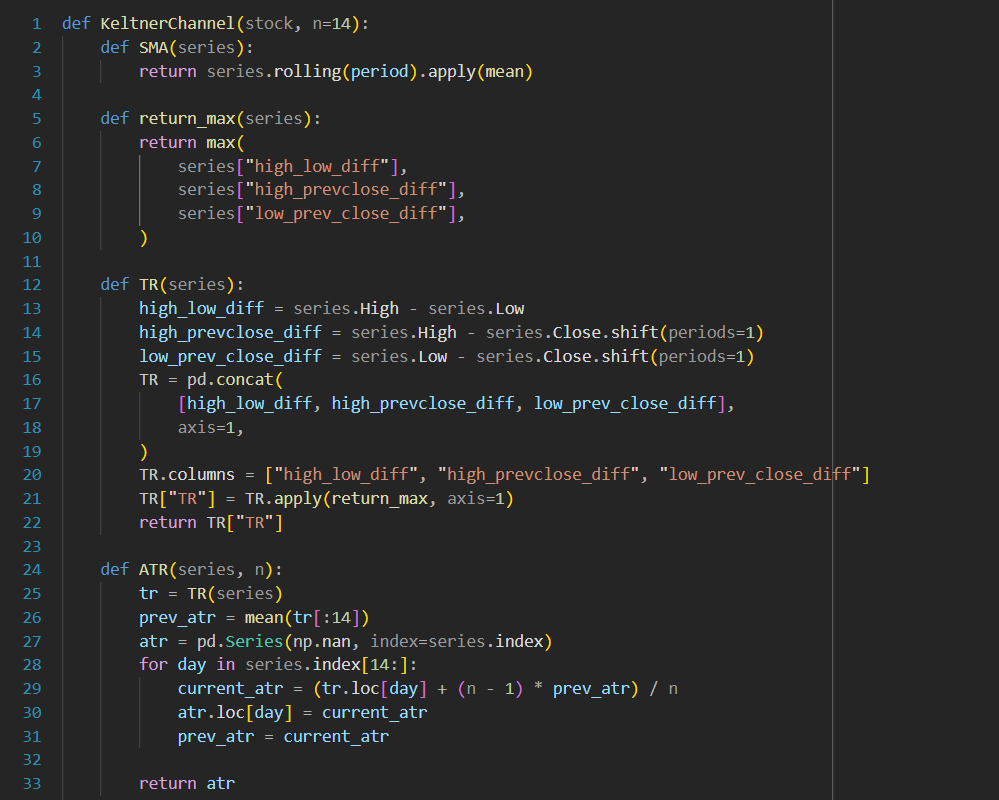
\includegraphics[height=6cm]{pic_6_1}}
	\quad \quad
	\subfloat[
	ادامه تابع اندیکاتور \lr{Keltner Channel}
	]{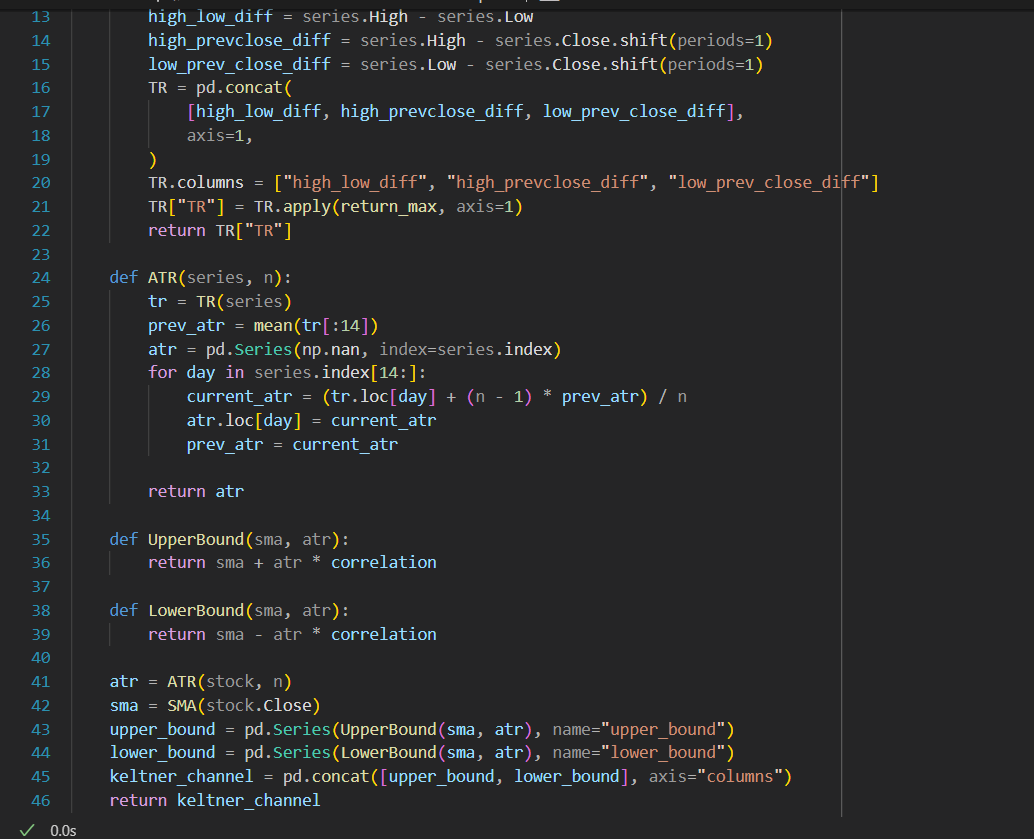
\includegraphics[height=6cm]{pic_6_2}}
\end{figure}
در تصویر زیر، اندیکاتور \lr{Keltner Channel} برای رمزارز \lr{BTC} با بازه‌های زمانی ۱ روزه محاسبه و ترسیم شده است.
\begin{figure}[H]
	\centering
	
\includegraphics[scale=0.5]{pic_7}
	\caption{اندیکاتور \lr{Keltner Channel} برای رمزارز \lr{BTC} در بازه‌های زمانی ۱ روزه}
\end{figure}
سپس به پیاده‌سازی \lr{RSI} می‌پردازیم. 
\begin{eqnarray*}
	RS &=& \frac{average\ gain}{average\ loss}\\
	RSI &=& 100 - \frac{100}{1 + RS}
\end{eqnarray*}
\begin{figure}[H]
	\centering
	
\includegraphics[scale=0.5]{pic_8}
\end{figure}
\lr{RSI} محاسبه شده برای رمزارز \lr{ETH} با بازه‌های زمانی ۱ روزه
\begin{figure}[H]
	\centering
	
\includegraphics[scale=0.5]{pic_9}
\end{figure}
\end{document}